\documentclass[12pt]{article}
\usepackage{authblk}
\usepackage{upgreek}
\usepackage{multirow}
\usepackage{indentfirst}
\usepackage{setspace}
\usepackage{geometry}
\usepackage{graphicx}
\usepackage{newtxtext, newtxmath}
\usepackage{listings}
\usepackage[usenames,dvipsnames]{color}

\definecolor{DarkGreen}{rgb}{0.0,0.4,0.0}

\lstloadlanguages{Matlab}
\lstset{breaklines}
\lstset{language=Matlab,
        frame=single,                           % single framed
        basicstyle=\small\ttfamily,
        keywordstyle=[1]\color{Blue}\bfseries,  % primitive funs in bold blue
        keywordstyle=[2]\color{Purple},         % args of funs in purple
        keywordstyle=[3]\color{Blue}\underbar,  % user funs in blue with underbar
        stringstyle=\color{Purple},             % strings in purple
        showstringspaces=false,
        identifierstyle=,
        commentstyle=\usefont{T1}{pcr}{m}{sl}\color{DarkGreen}\small,
        tabsize=4,
        % more standard MATLAB funcs
        morekeywords={sawtooth, square},
        % args of funcs
        morekeywords=[2]{on, off, interp},
        % user funcs
        morekeywords=[3]{FindESS, homework_example},
        morecomment=[l][\color{Blue}]{...},     % line continuation (...) like blue comment
        numbers=left,
        numberstyle=\tiny\color{Blue},
        firstnumber=1,
        stepnumber=1
        }
\geometry{a4paper,left=2.45cm,right=2.45cm,top=2.45cm,bottom=2.45cm}
\title{\huge Design and Analysis of a Laminated Composite Tube}
\author{Jiatai Deng, Jiawei Shuang, Xuanye Hu}
\affil{Department of Mechanical, Aerospace and Civil Engineering}
\date{\today}
\newpage
\begin{document}
\newpage
\maketitle
\thispagestyle{empty}
\newpage
\tableofcontents
\thispagestyle{empty} 
\newpage

\section{General description and requirement}
\setcounter{page}{1}
\pagenumbering{arabic}
\onehalfspacing
\noindent A cylindrical tube of 4 layers of composite with a layup of 
$\left[\alpha\  \beta\  \alpha\  \beta\right]$is to be designed and by winding tapes cut from a UD carbon-epoxy prepreg sheet on to a cylindrical mandrel of a 25mm radius. For the consideration of practicality, the range of these two winding angles will have to fall in [-75°, -30°] or [+30°, +75°] to the axis of the tube. The thickness of the prepreg is 0.25mm. The tube should be made to a length of 300mm.  \newline
\noindent \textbf{Material properties:}\newline
Internal pressure: $q = 3\times10^{6}$ \qquad Axial force: $P = 25 kN$ \newline
Tube radius: $R = 25\times10^{-3}$ \qquad  Tube length $L = 0.3$ \newline
Elastic constant: $E1 = 236 GPa$ \qquad $E2 = 5 GPa$ \qquad $G = 2.6 GPa$ \qquad $\upsilon_{12} = 0.25 GPa$ \newline
Strengths: $\sigma_{1t}^{*} = 3800 MPa$ \qquad $\sigma_{2t}^{*} = 41 MPa$ \qquad $\sigma_{1c}^{*} = 689 MPa$ \qquad $\sigma_{2c}^{*} = 107 MPa$\qquad\qquad\qquad $\tau _{12}^{*} = 69 MPa$ 
\section{Design approach and theory}
\noindent The thickness of each layers is 0.25mm, thickness in the range is between 0.1~1.0 mm can be seen as lamina. So the developed tube is a laminate with layup: $[\alpha /\beta /\alpha /\beta ]$ and the laminate theory can be used for stress analysis.\newline\newline
\noindent \textbf{STEP I: Define the two winding angles:}\newline
\noindent According to the requirement, the winding angle of 4 layers can be defined:\newline
\begin{center}
$-75^{\circ} \leq \alpha \leq -30^{\circ}$ or $75^{\circ} \leq \alpha \leq 30^{\circ}$\end{center}
\begin{center}
$-75^{\circ} \leq \beta \leq -30^{\circ}$ or $75^{\circ} \leq \beta \leq 30^{\circ}$
\end{center}
\noindent \textbf{STEP II: Define the Stress-Strain Relationship $\left[ Q \right]$ :}\newline
According to the Laminar Stress-Strain Relationship in Material coordinate system: 
\begin{center}
	\begin{equation}
		\begin{align}
	&\left\{ \sigma \right\} = \left[Q \right] \left\{ \epsilon \right\} \\
&\left\{ \begin{matrix}
    \sigma_1  \\
    \sigma_2  \\
    \tau_{12}  \\
    \end{matrix} \right\} = \left[\begin{matrix}
		Q_{11} & Q_{12} & 0 \\
		Q_{12} & Q_{22} & 0 \\
		0 & 0 & Q_{66} \\
		\end{matrix} \right] \left\{ \begin{matrix}
			\epsilon_1  \\
			\epsilon_2  \\
			\gamma_{12}  \\
			\end{matrix} \right\} = \left[\begin{matrix}
				\frac{E1}{1-\upsilon^2\frac{E2}{E1}} & \frac{\Upsilon E2}{1-\upsilon^2\frac{E2}{E1}} & 0 \\
				\frac{\Upsilon E2}{1-\upsilon^2\frac{E2}{E1}} & \frac{E2}{1-\upsilon^2\frac{E2}{E1}} & 0 \\
				0 & 0 & G \\
				\end{matrix} \right] \left\{ \begin{matrix}
					\epsilon_1  \\
					\epsilon_2  \\
					\gamma_{12}  \\
					\end{matrix} \right\}
				\end{align}
				\end{equation}
			\end{center}\newline
\noindent \textbf{STEP III: Define the Coordinate transformation $\left[ T \right]$}\newline
\noindent The winding angle of 4 layers of composite: $ \theta = \left( \begin{matrix}
	\alpha  \\
	\beta  \\
	\alpha  \\
	\beta	\\
	\end{matrix} \right)$, the coordinate transformation between (x-y) and (1-2) matrix:
	\begin{center}
		\begin{equation}
			\begin{align}
				\left\{ T \right\} = \left[\begin{matrix}
			\cos^2{\theta} & \sin^2{\theta} & -2\cos{\theta}\sin{\theta} \\
			\sin^2{\theta} & \cos^2{\theta} & 2\cos{\theta}\sin{\theta} \\
			\cos{\theta}\sin{\theta} & -\cos{\theta}\sin{\theta} & cos^2{\theta}-sin^2{\theta} \\
			\end{matrix} \right]
		\end{align}
	\end{equation}
\end{center}\newline
\noindent \textbf{STEP IV: Define maximum stress failare criterion}\newline
\noindent According to the maximum stress failure criterion, material will fail when any of the following conditions is violated:
\begin{center}
	\begin{equation}
		\begin{align}
\frac{\sigma_1}{\sigma^*_{1t}} \leq 1 \quad if \quad \sigma_1 > 0 \qquad\qquad\qquad \frac{\left| \sigma_1 \right|}{\sigma^*_{1c}} \leq 1 \quad if \quad  \sigma_1 < 0 \\
\frac{\sigma_2}{\sigma^*_{2t}} \leq 1 \quad if \quad \sigma_2 > 0 \qquad\qquad\qquad \frac{\left| \sigma_2 \right|}{\sigma^*_{2c}} \leq 1 \quad if \quad  \sigma_2 < 0\\
\frac{\left| \tau_{12} \right|}{\tau^*_{12}} \leq 1\hfill\\
\end{align}
\end{equation}
\end{center}\newline
\noindent \textbf{STEP V: Define Twist angle}\newline
\noindent Tube is fixed at the bottom end and axially compressed at the top. Generator on the tube deforms by an angle $\gamma_{xy}$.
Point $A$ at the top end moves to $A'$ by a distance $\gamma_{xy}L$.
We can get the twist angle of the tube formula:\newline
\begin{center}
	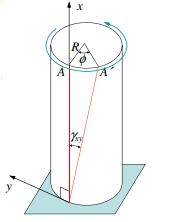
\includegraphics{twist.png}\newline
\end{center}
		\begin{equation}
			\begin{align}
	$$\theta = \frac{\gamma_{xy}L}{R}$$
\end{align}
\end{equation}
\noindent\textbf{There are two loading conditions, separately analysis:}\newline
\subsection{Case 1: Internal pressure of 3 MPa (ends closed)}
\begin{minipage}[c]{0.5\linewidth}
    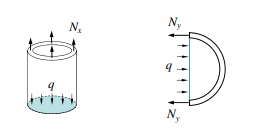
\includegraphics[scale=0.8]{case1.png}
\end{minipage}\hfill
\begin{minipage}[c]{0.5\linewidth}
	\noindent The generalised stresses:
	\begin{equation}
	 N = \left\{ \begin{matrix}
		N_x=\frac{1}{2}qR \\
		N_y=qR\newline  \\
		N_{xy}=0 
		\right\ }  \\
		\end{matrix} \right\}\\
	\end{equation}
\end{minipage}\hfill

\noindent Generalised stress-strain Relationship:
\begin{equation}
	\begin{align}
 \left\{\begin{matrix}
    N \\
    M \\
    \end{matrix}\right\}=&\left[\begin{matrix}
        A\ B\\
        B\ D\\\end{matrix}\right]\left\{\begin{matrix}
        \epsilon^0 \\
        \kappa \\
		\end{matrix}\right\}\\
		\left[A\right]=&\ t\left[T\right]\left[Q\right]\left[T\right]^T
	\end{align}
\end{equation}
Strain in x-direction: \begin{equation}
	\begin{align}
		\epsilon_x = \left[A\right]^{-1}N
	\end{align}
\end{equation}
\noindent \textbf{Lamina 1: The winding angle is $\alpha$.}\newline
\noindent In the STEP II, Stress-Strain Relationship has been defined:\newline
\begin{equation}
	\begin{align}
\epsilon_\alpha = \left[T_\alpha\right]\left[A\right]^{-1}^T\epsilon_x\qquad
\epsilon_\alpha=\left\{ \begin{matrix}
    \sigma_1  \\
    \sigma_2  \\
    \tau_{12}  \\
	\end{matrix} \right\}\qquad\sigma_\alpha=\left[Q\right]\epsilon_\alpha\qquad\sigma_\alpha=\left\{ \begin{matrix}
		\sigma_1  \\
		\sigma_2  \\
		\tau_{12}  \\
		\end{matrix} \right\}
	\end{align}
\end{equation}
\noindent Maximum stress failure criterion is given in step IV, substitute $\sigma$ into the formula to determine failure situation. And the results can indicate the failure modes, if $\frac{\left| \sigma_{1/2} \right|}{\sigma^*_{t/c}} \geq 1 $, this means Shear failure occurs, if $ \frac{\left| \tau_{12} \right|}{\tau^*_{12}} \geq 1 $,this means Transverse tensile failure occurs.\newline
\noindent \textbf{Lamina 2: The winding angle is $\beta$.}\newline
\noindent In the STEP II, Stress-Strain Relationship has been defined:
\begin{equation}
	\begin{align}
\epsilon_\beta = \left[T_\beta\right]\left[A\right]^{-1}^T\epsilon_x\qquad
\epsilon_\beta=\left\{ \begin{matrix}
    \sigma_1  \\
    \sigma_2  \\
    \tau_{12}  \\
	\end{matrix} \right\}\qquad\sigma_\beta=\left[Q\right]\epsilon_\beta\qquad\sigma_\beta=\left\{ \begin{matrix}
		\sigma_1  \\
		\sigma_2  \\
		\tau_{12}  \\
		\end{matrix} \right\}
	\end{align}
	\end{equation}\newline
\noindent Using the maximum stress failure criterion to indicate the failure modes as Lamina 1.
\subsection{Case 2:Axial compression of $P =25 kN$}
\begin{minipage}[c]{0.5\linewidth}
    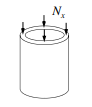
\includegraphics[scale=0.8]{case 2.png}
\end{minipage}\hfill
\begin{minipage}[c]{0.5\linewidth}
	\noindent The generalised stresses:
	\begin{equation}
	 N = \left\{ \begin{matrix}
		N_x=\frac{P}{2\pi R} \\
		N_y=0\newline  \\
		N_{xy}=0 
		\right\ }  \\
		\end{matrix} \right\}\\
	\end{equation}
\end{minipage}\hfill
\newline
\noindent Generalised stress-strain Relationship:
\begin{equation}
	\begin{align}
 \left\{\begin{matrix}
    N \\
    M \\
    \end{matrix}\right\}=&\left[\begin{matrix}
        A\ B\\
        B\ D\\\end{matrix}\right]\left\{\begin{matrix}
        \epsilon^0 \\
        \kappa \\
		\end{matrix}\right\}\\
		\left[A\right]=&\ t\left[T\right]\left[Q\right]\left[T\right]^T
	\end{align}
\end{equation}
Strain in x-direction: $\epsilon_x = \left[A\right]^{-1}N$\newline
\noindent The rest of the calculation method is the same as Case 1.
\subsection{The maximum angle of twist without failure}
\noindent Among all the winding angles which enable the tube to withstand the axial load and the internal pressure, there will be a set of angle values: $\alpha$\ and\ $\beta$ to make the tube get the maximum twist angle without failure.

\section{ Results and analysis to prove the success of the design }

\appendix
\section{Appendix}
\begin{lstlisting}
%%Unit: Pa,m%%
%%Term CASE1FM loading case 1 Failure matrix%%
%%Term CASE2FM loading case 2 Failure matrix%%
%%Term AssemblyFM Assembled Falure matrix [-30,30] has been removed%%
%%Term CASE2TA loading case 2 twist angle%%
%%Term BP Best point%%

format short %%Modify according to the requirement%%

%%Basic parameters%%

resolution=1; %%Modify according to the requirement%%
Delete=[0]; %%leave it alone%%
q=3e6;
P=-2.5e4;
R=25e-3; 
thick=2.5e-4;
L=0.3;
E1=236e9;
E2=5e9;
G=2.6e9;
v=0.25;
Xt=3800e6;
Xc=689e6;
Yt=41e6;
Yc=107e6;
S=69e6;
TAT_1=zeros(150/resolution+1); %%Initial matrix of Twist Angle%%
TAT_1=zeros(150/resolution+1);
for i=-75/resolution:1:75/resolution %%2 for loots control the Alpha and Beta%%
	Alpha=i*resolution;
	AlphaF=i+75/resolution+1;
	for i=-75/resolution:1:75/resolution
		Beta=i*resolution;
		BetaF=i+75/resolution+1;
		Theta=[Alpha;Beta;Alpha;Beta];
		t=[thick;thick;thick;thick];
		ctraQ=1-((v^2)*(E2/E1));
		Q=[E1/ctraQ v*E2/ctraQ 0; v*E2/ctraQ E2/ctraQ 0; 0 0 G];
		TT=[0;0;0];
			for i = 1:4 %%Find related equition in sheet%%
				straTAlpha=sind(Theta(i));
				ctraTAlpha=cosd(Theta(i));
				TAlpha=[ctraTAlpha^2 straTAlpha^2 -2*ctraTAlpha*straTAlpha;
				straTAlpha^2 ctraTAlpha^2 2*ctraTAlpha*straTAlpha;
				ctraTAlpha*straTAlpha -ctraTAlpha*straTAlpha ctraTAlpha^2-straTAlpha^2];
				TT=[TT TAlpha];
				eval(['TT',num2str(i),'=TAlpha;'])
			end
		TT=TT(:, 2:13);
		A=zeros(3);
			for i=1:4
				m=(i-1)*3+1;
				n=i*3;
				TTa=TT(:,m:n);
				A=A+thick*TTa*Q*TTa';
				Delete=Delete';
			end
		a=A^(-1);
		Q0=Q;

		%%Case one%%

		N_1=[0.5*q*R; q*R; 0];
		Epsilonx_1=a*N_1;
		Phi_1=Epsilonx_1(3)*L/R*180/pi;
		TAT1(AlphaF,BetaF)=Phi_1;
			for i=1:4
				m=(i-1)*3+1;
				n=i*3;
				TTa=TT(:,m:n);
				Epsilon_1= TTa'*Epsilonx_1;
				Delete=Delete';
				Sigma=Q0*Epsilon_1;
					if Sigma(1)>=0
						w1=Sigma(1)/Xt;
					else 
						w1=-Sigma(1)/Xc;
					end
					if Sigma(2)>=0
						w2=Sigma(2)/Yt;
					else
						w2=-Sigma(2)/Yc;	
					end
				w3=abs(Sigma(3)/S);
				w=[w1; w2; w3];
				eval(['wcone',num2str(i),'=w;'])
			end
		wwassembly_1=[wcone1 wcone2 wcone3 wcone4];	
		Fail_case_one_1=all(wwassembly_1(:)<=1);
		TATT_1(AlphaF,BetaF)=Fail_case_one_1;
		TATT_1=TATT_1*1;

		%%Case two%%

		N_2=[P/(2*pi*R); 0; 0];
		Epsilonx_2=a*N_2;
		Phi_2=Epsilonx_2(3)*L/R*180/pi;
		TAT_2(AlphaF,BetaF)=Phi_2;
			for i=1:4
				m=(i-1)*3+1;
				n=i*3;
				TTa=TT(:,m:n);
				Epsilon_2= TTa'*Epsilonx_2;
				Delete=Delete';
				Sigma=Q0*Epsilon_2;
					if Sigma(1)>=0
						w1=Sigma(1)/Xt;
					else 
						w1=-Sigma(1)/Xc;
					end
					if Sigma(2)>=0
						w2=Sigma(2)/Yt;
					else
						w2=-Sigma(2)/Yc;
					end
				w3=abs(Sigma(3)/S);
				w=[w1; w2; w3];
				eval(['wcone',num2str(i),'=w;'])
			end
		wwassembly_2=[wcone1 wcone2 wcone3 wcone4];
		Fail_case_one_2=all(wwassembly_2(:)<=1);
		TATT_2(AlphaF,BetaF)=Fail_case_one_2;
		TATT_2=TATT_2*1;
	end
end

CASE1FM=TATT_1;
XX=-75:resolution:75;
YY=-75:resolution:75;
CASE2FM=TATT_2;
CASE2TA=TAT_2;
CASE1FM((-30+75)/resolution+1:(30+75)/resolution+1,:)=0;
CASE1FM(:,(-30+75)/resolution+1:(30+75)/resolution+1)=0;

CASE2FM((-30+75)/resolution+1:(30+75)/resolution+1,:)=0;
CASE2FM(:,(-30+75)/resolution+1:(30+75)/resolution+1)=0;

%%Assemble the Failure matrix%%

AssemblyFM=CASE1FM.*CASE2FM;

%%Find the best point%%

TAFM=AssemblyFM.*CASE2TA;
BPZ=max(max(TAFM));
[BPX BPY]=find(TAFM==max(max(TAFM)));
BPX=(BPX(1)-1-75/resolution)*resolution;
BPY=(BPY(1)-1-75/resolution)*resolution;
BP=[BPX BPY BPZ]

%%0 become NAN for figure%%

ind=find(TAFM==0);  
TAFM(ind)=NaN;

%%Figure%%
	%%Colormap transformation%%

colormap(parula);

	%%TA Figure%%

mesh(XX,YY,CASE2TA);
title('Twist Angle','Fontname', 'Times New Roman','FontSize',24);
x1=xlabel('Alpha (degree)','Fontname', 'Times New Roman','FontSize',18);
x2=ylabel('Beta (degree)','Fontname', 'Times New Roman','FontSize',18);
x3=zlabel('Twist angle (degree)','Fontname', 'Times New Roman','FontSize',18);
set(x1,'Rotation',18);
set(x2,'Rotation',-25);

saveas(gcf,'Twist Angle.jpg');

	%%TA plane figure%%

contour(XX,YY,CASE2TA,10,'ShowText','on');
title('Twist Angle (degree)','Fontname', 'Times New Roman','FontSize',24);
x1=xlabel('Alpha (degree)','Fontname', 'Times New Roman','FontSize',18);
x2=ylabel('Beta (degree)','Fontname', 'Times New Roman','FontSize',18);

saveas(gcf,'Twist Angle (degree).jpg');

	%%TA Figure without Failure%%

mesh(XX,YY,TAFM);
title('Twist Angle without Failure','Fontname', 'Times New Roman','FontSize',24);
x1=xlabel('Alpha (degree)','Fontname', 'Times New Roman','FontSize',18);
x2=ylabel('Beta (degree)','Fontname', 'Times New Roman','FontSize',18);
x3=zlabel('Twist angle (degree)','Fontname', 'Times New Roman','FontSize',18);
set(x1,'Rotation',18);
set(x2,'Rotation',-25);

saveas(gcf,'Twist Angle without Failure.jpg');

	%%Colormap transformation%%

colormap(gray);

	%%Devided failure analysis figure%%

gca=pcolor(XX,YY,CASE1FM);
set(gca, 'LineStyle','none');
title('Failure Analysis of Case One','Fontname', 'Times New Roman','FontSize',24);
x1=xlabel('Alpha (degree)','Fontname', 'Times New Roman','FontSize',18);
x2=ylabel('Beta (degree)','Fontname', 'Times New Roman','FontSize',18);

saveas(gcf,'Failure Analysis of Case One.jpg');

gca=pcolor(XX,YY,CASE2FM);
set(gca, 'LineStyle','none');
title('Failure Analysis of Case Two','Fontname', 'Times New Roman','FontSize',24);
x1=xlabel('Alpha (degree)','Fontname', 'Times New Roman','FontSize',18);
x2=ylabel('Beta (degree)','Fontname', 'Times New Roman','FontSize',18);

saveas(gcf,'Failure Analysis of Case Two.jpg');

	%%Assembled failure analysis figure%%

gca=pcolor(XX,YY,AssemblyFM);
set(gca, 'LineStyle','none');
title('Failure Analysis','Fontname', 'Times New Roman','FontSize',24);
x1=xlabel('Alpha (degree)','Fontname', 'Times New Roman','FontSize',18);
x2=ylabel('Beta (degree)','Fontname', 'Times New Roman','FontSize',18);

saveas(gcf,'Failure Analysis.jpg');
	\end{lstlisting}
\end{document}